\documentclass[aspectratio=169]{beamer}

% Shared preamble for Claude Code slide decks
% Usage: % Shared preamble for Claude Code slide decks
% Usage: % Shared preamble for Claude Code slide decks
% Usage: \input{preamble} after \documentclass[aspectratio=169]{beamer}

\usetheme{default}
\usecolortheme{dove}

\setbeamertemplate{navigation symbols}{}
\setbeamertemplate{footline}{%
  \hfill{\large\insertframenumber\,/\,\inserttotalframenumber}\hspace{0.8em}\vspace{0.5em}%
}

\definecolor{popblue}{RGB}{52, 101, 164}
\definecolor{sampred}{RGB}{204, 0, 0}
\definecolor{paramgreen}{RGB}{0, 140, 70}
\definecolor{lightbg}{RGB}{245, 245, 250}
\definecolor{warnred}{RGB}{180, 40, 40}
\definecolor{orange1}{RGB}{220, 120, 0}
\definecolor{violet1}{RGB}{120, 50, 160}

\setbeamercolor{frametitle}{fg=popblue}
\setbeamercolor{title}{fg=popblue}
\setbeamercolor{block title}{fg=white,bg=popblue}
\setbeamercolor{block body}{bg=lightbg}
\setbeamercolor{block title alerted}{fg=white,bg=warnred}
\setbeamercolor{block body alerted}{bg=lightbg}
\setbeamercolor{block title example}{fg=white,bg=paramgreen}
\setbeamercolor{block body example}{bg=lightbg}

\usepackage{listings}
\usepackage[T1]{fontenc}
\usepackage{hyperref}
\usepackage{tikz}
\usepackage{booktabs}
\usetikzlibrary{shapes, arrows.meta, positioning, calc}

\lstset{
  basicstyle=\ttfamily\scriptsize,
  keywordstyle=\color{popblue}\bfseries,
  stringstyle=\color{paramgreen},
  commentstyle=\color{gray},
  breaklines=true,
  frame=single,
  backgroundcolor=\color{lightbg},
  rulecolor=\color{popblue!30},
  showstringspaces=false,
  columns=fullflexible,
}
 after \documentclass[aspectratio=169]{beamer}

\usetheme{default}
\usecolortheme{dove}

\setbeamertemplate{navigation symbols}{}
\setbeamertemplate{footline}{%
  \hfill{\large\insertframenumber\,/\,\inserttotalframenumber}\hspace{0.8em}\vspace{0.5em}%
}

\definecolor{popblue}{RGB}{52, 101, 164}
\definecolor{sampred}{RGB}{204, 0, 0}
\definecolor{paramgreen}{RGB}{0, 140, 70}
\definecolor{lightbg}{RGB}{245, 245, 250}
\definecolor{warnred}{RGB}{180, 40, 40}
\definecolor{orange1}{RGB}{220, 120, 0}
\definecolor{violet1}{RGB}{120, 50, 160}

\setbeamercolor{frametitle}{fg=popblue}
\setbeamercolor{title}{fg=popblue}
\setbeamercolor{block title}{fg=white,bg=popblue}
\setbeamercolor{block body}{bg=lightbg}
\setbeamercolor{block title alerted}{fg=white,bg=warnred}
\setbeamercolor{block body alerted}{bg=lightbg}
\setbeamercolor{block title example}{fg=white,bg=paramgreen}
\setbeamercolor{block body example}{bg=lightbg}

\usepackage{listings}
\usepackage[T1]{fontenc}
\usepackage{hyperref}
\usepackage{tikz}
\usepackage{booktabs}
\usetikzlibrary{shapes, arrows.meta, positioning, calc}

\lstset{
  basicstyle=\ttfamily\scriptsize,
  keywordstyle=\color{popblue}\bfseries,
  stringstyle=\color{paramgreen},
  commentstyle=\color{gray},
  breaklines=true,
  frame=single,
  backgroundcolor=\color{lightbg},
  rulecolor=\color{popblue!30},
  showstringspaces=false,
  columns=fullflexible,
}
 after \documentclass[aspectratio=169]{beamer}

\usetheme{default}
\usecolortheme{dove}

\setbeamertemplate{navigation symbols}{}
\setbeamertemplate{footline}{%
  \hfill{\large\insertframenumber\,/\,\inserttotalframenumber}\hspace{0.8em}\vspace{0.5em}%
}

\definecolor{popblue}{RGB}{52, 101, 164}
\definecolor{sampred}{RGB}{204, 0, 0}
\definecolor{paramgreen}{RGB}{0, 140, 70}
\definecolor{lightbg}{RGB}{245, 245, 250}
\definecolor{warnred}{RGB}{180, 40, 40}
\definecolor{orange1}{RGB}{220, 120, 0}
\definecolor{violet1}{RGB}{120, 50, 160}

\setbeamercolor{frametitle}{fg=popblue}
\setbeamercolor{title}{fg=popblue}
\setbeamercolor{block title}{fg=white,bg=popblue}
\setbeamercolor{block body}{bg=lightbg}
\setbeamercolor{block title alerted}{fg=white,bg=warnred}
\setbeamercolor{block body alerted}{bg=lightbg}
\setbeamercolor{block title example}{fg=white,bg=paramgreen}
\setbeamercolor{block body example}{bg=lightbg}

\usepackage{listings}
\usepackage[T1]{fontenc}
\usepackage{hyperref}
\usepackage{tikz}
\usepackage{booktabs}
\usetikzlibrary{shapes, arrows.meta, positioning, calc}

\lstset{
  basicstyle=\ttfamily\scriptsize,
  keywordstyle=\color{popblue}\bfseries,
  stringstyle=\color{paramgreen},
  commentstyle=\color{gray},
  breaklines=true,
  frame=single,
  backgroundcolor=\color{lightbg},
  rulecolor=\color{popblue!30},
  showstringspaces=false,
  columns=fullflexible,
}


\title{Claude Code Workflow Tricks}
\subtitle{Plugins $\cdot$ Skills $\cdot$ Hooks $\cdot$ MCPs $\cdot$ Patterns for Power Users}
\author{mostly Opus 4.6}
\date{}

\begin{document}

% ──────────────────────────────────────────────
\begin{frame}
\titlepage
\end{frame}

% ──────────────────────────────────────────────
\begin{frame}{What This Deck Covers}
\begin{columns}[T]
\column{0.33\textwidth}
\textbf{\color{popblue}Environment}
\begin{itemize}
  \item CLI vs.\ IDE terminal
  \item Terminal \& shortcut setup
  \item ccstatusline
\end{itemize}

\bigskip
\textbf{\color{paramgreen}Workflow Patterns}
\begin{itemize}
  \item Plan-review-code-review
  \item Project prompts \& self-improvement
  \item Autoresearch (Karpathy)
\end{itemize}

\column{0.33\textwidth}
\textbf{\color{orange1}Plugins}
\begin{itemize}
  \item Caveman (token savings)
  \item Superpowers (structured dev)
  \item MemPalace (persistent memory)
  \item Code review \& simplify
  \item Sequential thinking
\end{itemize}

\bigskip
\textbf{\color{violet1}Skills \& Subagents}
\begin{itemize}
  \item Built-in \& scientific skills
  \item Custom subagents
\end{itemize}

\column{0.33\textwidth}
\textbf{\color{warnred}Integrations}
\begin{itemize}
  \item Context7, Playwright, GitHub
  \item Hooks for safety
  \item Remote control
  \item Piping \& worktrees
  \item Personal setup (Gmail, Calendar, Telegram, \ldots)
\end{itemize}
\end{columns}

\vfill
\centering
\small Target audience: \textbf{you already use AI agents}. This is about leveling up.
\end{frame}

% ══════════════════════════════════════════════
% SECTION 1: Environment
% ══════════════════════════════════════════════
\section{Environment}

\begin{frame}{CLI vs.\ IDE Terminal}
\begin{columns}[T]
\column{0.48\textwidth}
\textbf{\color{popblue}CLI wins for heavy work}
\begin{itemize}
  \item Auto model selection for reasoning tasks
  \item Full terminal visibility (scrollback, width)
  \item \texttt{Shift+Tab} permission cycling
  \item Background tasks (\texttt{Ctrl+B})
  \item Voice mode (\texttt{/voice})
  \item Piping: \texttt{cat file | claude -p "..."}
  \item Remote control (\texttt{/rc})
\end{itemize}

\column{0.48\textwidth}
\textbf{\color{paramgreen}IDE wins for focused edits}
\begin{itemize}
  \item Inline diffs with side-by-side review
  \item \texttt{Alt+K} auto-inserts \texttt{@file\#lines}
  \item Multiple conversation tabs
  \item Rewind with visual checkpoints
  \item See changes in context of surrounding code
\end{itemize}

\bigskip
\begin{exampleblock}{Recommendation}
CLI for orchestration \& long tasks. \\
IDE for file-focused edits \& review.
\end{exampleblock}
\end{columns}
\end{frame}

% ──────────────────────────────────────────────
\begin{frame}{Terminal \& Shortcut Setup}
\begin{columns}[T]
\column{0.5\textwidth}
\textbf{\color{popblue}Claude Code shortcuts}
\begin{itemize}\setlength\itemsep{0.15em}
  \item \texttt{Shift+Tab} --- cycle permission modes
  \item \texttt{Esc} --- stop, redirect
  \item \texttt{Esc+Esc} --- rewind to checkpoint
  \item \texttt{Ctrl+O} --- toggle verbose (see thinking)
  \item \texttt{Ctrl+B} --- background a task
  \item \texttt{Ctrl+G} --- open prompt in editor
  \item \texttt{Ctrl+R} --- search command history
  \item \texttt{/vim} --- enable vim keybindings
\end{itemize}

\column{0.5\textwidth}
\textbf{\color{paramgreen}VS Code terminal tips}
\begin{itemize}\setlength\itemsep{0.15em}
  \item Use a Nerd Font for ccstatusline icons
  \item Increase scrollback: \texttt{terminal.integrated.scrollback: 10000}
  \item Watch for \texttt{Ctrl+B} conflict (toggle sidebar)
  \item Remap or disable VS Code shortcuts that clash
\end{itemize}

\bigskip
\textbf{\color{orange1}Bash essentials}
\begin{itemize}\setlength\itemsep{0.15em}
  \item \texttt{!!} --- repeat last command
  \item \texttt{Ctrl+R} --- reverse history search
  \item \texttt{Ctrl+L} --- clear screen
  \item \texttt{Ctrl+A/E} --- jump to start/end of line
\end{itemize}
\end{columns}
\end{frame}

% ══════════════════════════════════════════════
% SECTION 2: Workflow Patterns
% ══════════════════════════════════════════════
\section{Workflow Patterns}

\begin{frame}{The Plan-Review-Code-Review Workflow}
\begin{center}
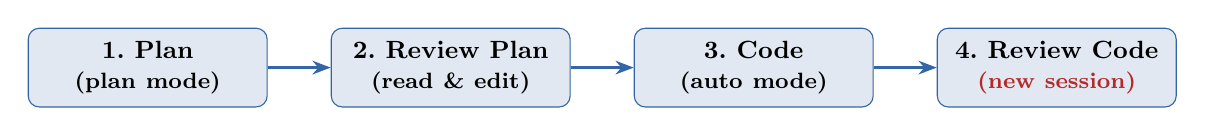
\begin{tikzpicture}[
  node distance=0.5cm and 0.8cm,
  phase/.style={rectangle, rounded corners, draw=popblue, fill=popblue!15,
                text width=2.8cm, minimum height=1cm, align=center, font=\small\bfseries},
  note/.style={font=\scriptsize, text width=2.8cm, align=center},
  arr/.style={-Stealth, thick, popblue}
]
  \node[phase] (plan) {1.\ Plan\\{\footnotesize(plan mode)}};
  \node[phase, right=of plan] (review1) {2.\ Review Plan\\{\footnotesize(read \& edit)}};
  \node[phase, right=of review1] (code) {3.\ Code\\{\footnotesize(auto mode)}};
  \node[phase, right=of code] (review2) {4.\ Review Code\\{\footnotesize\color{warnred}(new session)}};
  \draw[arr] (plan) -- (review1);
  \draw[arr] (review1) -- (code);
  \draw[arr] (code) -- (review2);
\end{tikzpicture}
\end{center}

\begin{columns}[T]
\column{0.5\textwidth}
\textbf{\color{popblue}Why separate sessions?}
\begin{itemize}
  \item Fresh context = fresh eyes
  \item No accumulated bias from coding phase
  \item Reviewer catches what the author missed
\end{itemize}

\column{0.5\textwidth}
\textbf{\color{paramgreen}In practice}
\begin{itemize}
  \item \texttt{claude -n "impl-auth"} for coding
  \item \texttt{claude -n "review-auth"} for review
  \item Or: \texttt{/code-review} plugin (4 parallel agents)
\end{itemize}
\end{columns}

\smallskip
\begin{alertblock}{Rule}
Never skip the plan phase for non-trivial tasks. A 2-minute plan saves 20 minutes of rework.
\end{alertblock}
\end{frame}

% ──────────────────────────────────────────────
\begin{frame}{Project Prompts \& Self-Improvement}
\begin{columns}[T]
\column{0.5\textwidth}
\textbf{\color{popblue}Set up the project context}
\begin{itemize}
  \item Write a clear \texttt{CLAUDE.md} (under 200 lines)
  \item Describe architecture, constraints, conventions
  \item Include build/test commands Claude can't guess
  \item Use \texttt{.claude/rules/*.md} for path-specific rules
\end{itemize}

\bigskip
\textbf{\color{paramgreen}Track progress}
\begin{itemize}
  \item ``Keep track of your progress as you go''
  \item ``Save what you learned to memory''
  \item Name sessions: \texttt{claude -n "feature-X"}
\end{itemize}

\column{0.5\textwidth}
\textbf{\color{orange1}The meta-improvement loop}

Periodically ask Claude:
\begin{itemize}
  \item ``What workflow improvements would you suggest for this project?''
  \item ``Review my CLAUDE.md --- what's redundant or missing?''
  \item ``What hooks or skills would make our workflow better?''
  \item ``What patterns in my usage should I automate?''
\end{itemize}

\begin{exampleblock}{Highest-leverage trick}
Claude improves its own setup. \\
Let it audit and optimize your workflow.
\end{exampleblock}
\end{columns}
\end{frame}

% ──────────────────────────────────────────────
\begin{frame}{The Autoresearch Pattern (Karpathy)}
\begin{center}
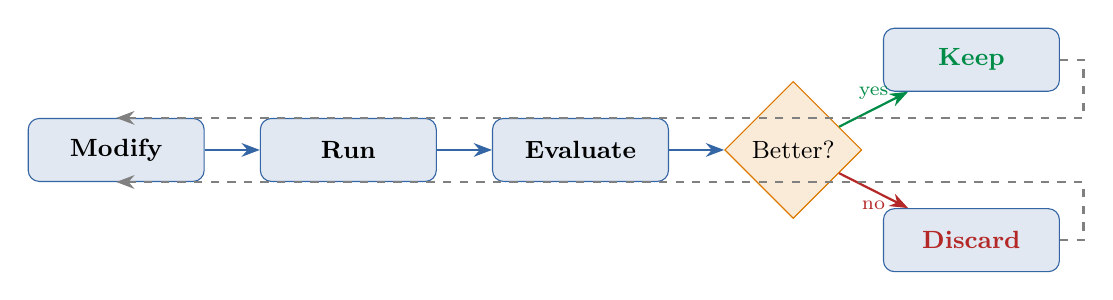
\begin{tikzpicture}[
  node distance=0.4cm and 0.7cm,
  phase/.style={rectangle, rounded corners, draw=popblue, fill=popblue!15,
                text width=2cm, minimum height=0.8cm, align=center, font=\small\bfseries},
  decision/.style={diamond, draw=orange1, fill=orange1!15,
                   minimum width=1.5cm, minimum height=1cm, align=center, font=\small},
  arr/.style={-Stealth, thick, popblue}
]
  \node[phase] (modify) {Modify};
  \node[phase, right=of modify] (run) {Run};
  \node[phase, right=of run] (eval) {Evaluate};
  \node[decision, right=of eval] (keep) {Better?};
  \node[phase, above right=0.3cm and 0.7cm of keep] (save) {\color{paramgreen}Keep};
  \node[phase, below right=0.3cm and 0.7cm of keep] (discard) {\color{warnred}Discard};
  \draw[arr] (modify) -- (run);
  \draw[arr] (run) -- (eval);
  \draw[arr] (eval) -- (keep);
  \draw[arr, paramgreen] (keep) -- node[above, font=\scriptsize] {yes} (save);
  \draw[arr, warnred] (keep) -- node[below, font=\scriptsize] {no} (discard);
  \draw[arr, dashed, gray] (save.east) -- ++(0.3,0) |- (modify.north);
  \draw[arr, dashed, gray] (discard.east) -- ++(0.3,0) |- (modify.south);
\end{tikzpicture}
\end{center}

\begin{columns}[T]
\column{0.5\textwidth}
\textbf{\color{popblue}What it is}
\begin{itemize}
  \item Give Claude a measurable task + evaluation metric
  \item Let it experiment autonomously overnight
  \item Keep improvements, discard regressions
  \item \href{https://github.com/karpathy/autoresearch}{\texttt{github.com/karpathy/autoresearch}} (72k+ stars)
\end{itemize}

\column{0.5\textwidth}
\textbf{\color{paramgreen}Results}
\begin{itemize}
  \item First overnight run: 83 experiments
  \item 15 improvements kept
  \item 11\% reduction in time-to-GPT-2
  \item Generalizable: any task with a measurable quality metric
\end{itemize}
\end{columns}
\end{frame}

% ══════════════════════════════════════════════
% SECTION 3: Plugins
% ══════════════════════════════════════════════
\section{Plugins}

\begin{frame}[fragile]{Caveman Plugin}
\textbf{Cut $\sim$75\% output tokens} by stripping filler while keeping full technical accuracy.

\smallskip
\textbf{Install:}
\begin{lstlisting}[language=bash]
claude plugin marketplace add JuliusBrussee/caveman
claude plugin install caveman@caveman
\end{lstlisting}

\begin{columns}[T]
\column{0.5\textwidth}
\textbf{\color{popblue}Three compression levels}
\begin{itemize}
  \item \texttt{/caveman lite} --- drops filler, keeps grammar
  \item \texttt{/caveman full} --- fragments, drops articles
  \item \texttt{/caveman ultra} --- maximum telegraphic compression
\end{itemize}

\column{0.5\textwidth}
\textbf{\color{paramgreen}Why it matters}
\begin{itemize}
  \item Research: brevity constraints improved accuracy by 26 percentage points
  \item Terse commits, one-line code reviews
  \item Input compression too ($\sim$46\% savings)
  \item \href{https://github.com/JuliusBrussee/caveman}{\texttt{github.com/JuliusBrussee/caveman}}
\end{itemize}
\end{columns}
\end{frame}

% ──────────────────────────────────────────────
\begin{frame}[fragile]{Superpowers Plugin}
\textbf{Enforced 5-phase development workflow} with TDD and subagent-driven code.

\smallskip
\textbf{Install:}
\begin{lstlisting}[language=bash]
/plugin install superpowers@claude-plugins-official
\end{lstlisting}

\begin{columns}[T]
\column{0.55\textwidth}
\textbf{\color{popblue}The 5 phases}
\begin{enumerate}
  \item \textbf{Clarify} requirements
  \item \textbf{Design} architecture
  \item \textbf{Plan} implementation steps
  \item \textbf{Code} with TDD (red-green-refactor)
  \item \textbf{Verify} with two-stage review
\end{enumerate}

\column{0.42\textwidth}
\textbf{\color{paramgreen}Key features}
\begin{itemize}
  \item Subagent-driven development
  \item Git worktree isolation
  \item Systematic debugging with root-cause analysis
  \item 153k+ stars on GitHub
  \item By Jesse Vincent (\texttt{obra})
\end{itemize}
\end{columns}

\begin{alertblock}{Why use it}
Prevents the ``just start coding'' failure mode. Forces you to think before you type.
\end{alertblock}
\end{frame}

% ──────────────────────────────────────────────
\begin{frame}[fragile]{MemPalace}
\textbf{Local-first AI memory} with 96.6\% recall --- zero API calls, 100\% on your machine.

\smallskip
\textbf{Install:}
\begin{lstlisting}[language=bash]
pip install mempalace
\end{lstlisting}

\begin{columns}[T]
\column{0.5\textwidth}
\textbf{\color{popblue}How it works}
\begin{itemize}
  \item \textbf{Verbatim storage} --- no lossy summarization
  \item Method of loci: Wings $\to$ Rooms $\to$ Halls $\to$ Closets $\to$ Drawers
  \item 29 MCP tools for palace read/write, knowledge graph, agent diaries
  \item Auto-save hooks before context compression
\end{itemize}

\column{0.5\textwidth}
\textbf{\color{paramgreen}Why not built-in memory?}
\begin{itemize}
  \item Built-in memory is flat markdown files
  \item MemPalace: temporal knowledge graph with validity windows
  \item Cross-session, cross-project recall
  \item 96.6\% on LongMemEval benchmark
  \item \href{https://github.com/MemPalace/mempalace}{\texttt{github.com/MemPalace/mempalace}}
\end{itemize}
\end{columns}
\end{frame}

% ──────────────────────────────────────────────
\begin{frame}[fragile]{Code Review, Simplify \& Sequential Thinking}
\begin{columns}[T]
\column{0.5\textwidth}
\textbf{\color{popblue}Code Review plugin} {\small(Anthropic, free)}
\begin{itemize}
  \item \texttt{/code-review} runs 4 parallel agents
  \item CLAUDE.md compliance, bug scan, git-blame context
  \item Findings scored 0--100, threshold filters noise
  \item Install: \texttt{/plugin install code-review}
\end{itemize}

\medskip
\textbf{\color{paramgreen}Code Simplify} {\small(built-in)}
\begin{itemize}
  \item \texttt{/simplify} --- post-implementation cleanup
  \item Preserves functionality, improves clarity
  \item Best workflow: code $\to$ \texttt{/code-review} $\to$ \texttt{/simplify}
\end{itemize}

\column{0.5\textwidth}
\textbf{\color{orange1}Sequential Thinking MCP}
\begin{itemize}
  \item Structured step-by-step reasoning
  \item Best for: architecture decisions, scope discovery, multi-step planning
  \item Reported 60--70\% time savings on complex features
\end{itemize}

\smallskip
\textbf{Setup:}
\begin{lstlisting}[language=bash]
claude mcp add seq-think \
  -- npx -y \
  @modelcontextprotocol/\
  server-sequential-thinking
\end{lstlisting}
\end{columns}
\end{frame}

% ══════════════════════════════════════════════
% SECTION 4: Skills & Subagents
% ══════════════════════════════════════════════
\section{Skills \& Subagents}

\begin{frame}{Skills That Matter}
\begin{columns}[T]
\column{0.5\textwidth}
\textbf{\color{popblue}Built-in skills}
\begin{itemize}
  \item \texttt{/batch} --- process multiple files
  \item \texttt{/simplify} --- clean up code
  \item \texttt{/debug} --- systematic debugging
  \item \texttt{/claude-api} --- Anthropic SDK help
  \item \texttt{/code-review} --- parallel review agents
\end{itemize}

\bigskip
\textbf{\color{paramgreen}Custom skills}
\begin{itemize}
  \item Write in \texttt{.claude/skills/*.md}
  \item Frontmatter: name, description, tools, model
  \item \texttt{user-invocable: true} to show in \texttt{/} menu
  \item Share via git or plugins
\end{itemize}

\column{0.5\textwidth}
\textbf{\color{orange1}Scientific Research Skills}

\href{https://github.com/K-Dense-AI/scientific-agent-skills}{\texttt{K-Dense-AI/scientific-agent-skills}}

133 ready-to-use skills:
\begin{itemize}
  \item Genomics \& bioinformatics
  \item Drug discovery \& cheminformatics
  \item Clinical research \& medical imaging
  \item Materials science \& physics
  \item Finance \& quantitative analysis
  \item 100+ scientific databases
\end{itemize}

\medskip
\textbf{\color{violet1}Open standard}
\begin{itemize}
  \item \href{https://agentskills.io}{\texttt{agentskills.io}}
  \item Works in Claude Code, Cursor, Codex, Gemini CLI
\end{itemize}
\end{columns}
\end{frame}

% ──────────────────────────────────────────────
\begin{frame}{Subagents for Parallel Work}
\begin{columns}[T]
\column{0.5\textwidth}
\textbf{\color{popblue}Built-in subagents}
\begin{itemize}
  \item \textbf{Explore} --- codebase search
  \item \textbf{Plan} --- design implementation
  \item \textbf{General Purpose} --- any task
\end{itemize}

\bigskip
\textbf{\color{paramgreen}Custom agents}
\begin{itemize}
  \item Create \texttt{.claude/agents/reviewer.md}
  \item Frontmatter: tools, model, isolation
  \item \texttt{isolation: worktree} for safe parallel dev
  \item \texttt{background: true} for async work
\end{itemize}

\column{0.5\textwidth}
\textbf{\color{orange1}Invocation methods}
\begin{itemize}
  \item Natural language (auto-delegation)
  \item \texttt{@"reviewer (agent)"} (explicit)
  \item \texttt{claude --agent reviewer} (session-wide)
  \item \texttt{Ctrl+B} to background a running task
\end{itemize}

\bigskip
\begin{exampleblock}{Power pattern}
One subagent implements. \\
Another reviews in a worktree. \\
Main session merges results.
\end{exampleblock}
\end{columns}
\end{frame}

% ══════════════════════════════════════════════
% SECTION 5: MCPs
% ══════════════════════════════════════════════
\section{MCPs \& Integrations}

\begin{frame}[fragile]{Essential MCPs}
\begin{columns}[T]
\column{0.5\textwidth}
\textbf{\color{popblue}Context7} --- live library docs
\begin{lstlisting}[language=bash]
claude mcp add context7 \
  -- npx -y \
  @upstash/context7-mcp@latest
\end{lstlisting}
Say ``use context7'' $\to$ current API docs, no hallucination.

\bigskip
\textbf{\color{paramgreen}Playwright} --- browser control
\begin{lstlisting}[language=bash]
claude mcp add playwright \
  npx @playwright/mcp@latest
\end{lstlisting}
Automated testing, screenshots, form filling.

\column{0.5\textwidth}
\textbf{\color{orange1}GitHub} --- repo integration
\begin{itemize}
  \item \texttt{/install-github-app}
  \item \texttt{@claude} in issues/PRs
  \item Auto PR reviews
  \item Custom instructions per repo
\end{itemize}

\bigskip
\textbf{\color{violet1}Deferred tool loading}
\begin{itemize}
  \item MCP tools lazy-load via \texttt{ToolSearch}
  \item Hundreds of tools without context bloat
  \item Only loaded when actually needed
\end{itemize}
\end{columns}
\end{frame}

% ══════════════════════════════════════════════
% SECTION 6: Hooks
% ══════════════════════════════════════════════
\section{Hooks}

\begin{frame}[fragile]{Hooks for Safety \& Automation}
\begin{columns}[T]
\column{0.5\textwidth}
\textbf{\color{warnred}Safety hooks (PreToolUse)}
\begin{itemize}
  \item \textbf{No force-push}: block \texttt{git push --force}
  \item \textbf{No credentials}: block reads of \texttt{.env}, \texttt{credentials.json}
  \item \textbf{No production}: block deploys to prod
  \item Exit code 2 = blocked with message
\end{itemize}

\bigskip
\textbf{\color{paramgreen}Automation hooks (PostToolUse)}
\begin{itemize}
  \item Auto-format after edits (Prettier, Black)
  \item Run tests on changed files
  \item HTTP hook: POST to Slack on completion
\end{itemize}

\column{0.5\textwidth}
\textbf{\color{popblue}Startup briefing (SessionStart)}
\begin{lstlisting}[]
"SessionStart": [{
  "hooks": [{
    "type": "command",
    "command": "node briefing.js"
  }]
}]
\end{lstlisting}
Print today's tasks, open PRs, failing tests --- every time you start.

\medskip
{\small\textbf{\color{orange1}Config:} \texttt{.claude/settings.json} (team) $|$
\texttt{settings.local.json} (personal) $|$
\texttt{\textasciitilde/.claude/settings.json} (global)}
\end{columns}
\end{frame}

% ══════════════════════════════════════════════
% SECTION 7: More Tricks
% ══════════════════════════════════════════════
\section{More Tricks}

\begin{frame}[fragile]{More Tricks}
\begin{columns}[T]
\column{0.5\textwidth}
\textbf{\color{popblue}ccstatusline}
\begin{itemize}
  \item Beautiful status bar: model, git branch, tokens, timer
  \item Powerline themes, custom widgets
  \item \texttt{npx -y ccstatusline@latest}
  \item \href{https://github.com/sirmalloc/ccstatusline}{\texttt{github.com/sirmalloc/ccstatusline}}
\end{itemize}

\bigskip
\textbf{\color{paramgreen}Piping \& scripting}
\begin{lstlisting}[language=bash]
cat error.log | claude -p \
  "explain root cause" > out.txt
\end{lstlisting}
Headless mode for automation, grading scripts, batch processing.

\column{0.5\textwidth}
\textbf{\color{orange1}Git worktrees}
\begin{itemize}
  \item \texttt{claude --worktree feature-auth}
  \item Isolated repo copy per task
  \item No file conflicts between parallel tasks
\end{itemize}

\bigskip
\textbf{\color{violet1}Path-specific rules}
\begin{itemize}
  \item \texttt{.claude/rules/testing.md}
  \item Loads only when test files are edited
  \item Keep CLAUDE.md lean, rules specific
\end{itemize}

\bigskip
\textbf{\color{warnred}Remote control}
\begin{itemize}
  \item \texttt{/rc} --- continue from phone/browser
  \item That's it. One command.
\end{itemize}
\end{columns}
\end{frame}

% ══════════════════════════════════════════════
% SECTION 8: Personal Setup
% ══════════════════════════════════════════════
\section{Personal Setup}

\begin{frame}{Personal Setup: Your AI Assistant}
\begin{columns}[T]
\column{0.5\textwidth}
\textbf{\color{popblue}Communication}
\begin{itemize}
  \item \textbf{Gmail} --- read, draft, search emails
  \item \textbf{Telegram} --- reply, send files, reactions
  \item \textbf{Notion} --- search, create pages, manage databases
\end{itemize}

\bigskip
\textbf{\color{paramgreen}Productivity}
\begin{itemize}
  \item \textbf{Google Calendar} --- create events, list schedule, suggest meeting times
  \item \textbf{Google Drive} --- read, search, create files
\end{itemize}

\column{0.5\textwidth}
\textbf{\color{orange1}How it works}
\begin{itemize}
  \item All via MCP connections
  \item Runs 100\% locally
  \item Data stays on your machine
  \item OAuth authentication (one-time setup)
  \item Available in CLI and IDE
\end{itemize}

\bigskip
\begin{exampleblock}{Example workflow}
``Check my calendar for tomorrow, draft an email to Alex about the 3pm meeting, and create a Notion page with the agenda.''
\end{exampleblock}
\end{columns}
\end{frame}

% ══════════════════════════════════════════════
% Closing
% ══════════════════════════════════════════════

\begin{frame}{Summary}
\begin{columns}[T]
\column{0.5\textwidth}
\begin{block}{Workflow Upgrades}
\begin{itemize}
  \item Plan $\to$ review $\to$ code $\to$ review (separate session)
  \item Project prompts + memory updates
  \item Ask Claude to improve your workflow
  \item Autoresearch for measurable tasks
  \item \texttt{/code-review} $\to$ \texttt{/simplify} loop
\end{itemize}
\end{block}

\column{0.5\textwidth}
\begin{block}{Tools \& Integrations}
\begin{itemize}
  \item Caveman (75\% fewer tokens)
  \item Superpowers (structured dev)
  \item MemPalace (persistent memory)
  \item Sequential Thinking MCP
  \item Context7, Playwright, GitHub
  \item Hooks for safety \& automation
  \item Personal MCPs (Gmail, Calendar, \ldots)
\end{itemize}
\end{block}
\end{columns}

\vfill
\centering
{\Large\color{popblue} The best prompt is a well-structured workflow.}
\end{frame}

% ──────────────────────────────────────────────
\begin{frame}{Resources}
\small
\begin{columns}[T]
\column{0.5\textwidth}
\textbf{\color{popblue}Plugins \& Tools}
\begin{itemize}\setlength\itemsep{0.15em}
  \item \href{https://github.com/JuliusBrussee/caveman}{\textbf{Caveman}} --- token compression
  \item \href{https://github.com/obra/superpowers}{\textbf{Superpowers}} --- structured dev
  \item \href{https://github.com/MemPalace/mempalace}{\textbf{MemPalace}} --- persistent memory
  \item \href{https://github.com/sirmalloc/ccstatusline}{\textbf{ccstatusline}} --- custom status bar
  \item \href{https://github.com/karpathy/autoresearch}{\textbf{Autoresearch}} --- Karpathy's experiment loop
\end{itemize}

\medskip
\textbf{\color{paramgreen}Skills \& Standards}
\begin{itemize}\setlength\itemsep{0.15em}
  \item \href{https://github.com/K-Dense-AI/scientific-agent-skills}{\textbf{Scientific Agent Skills}} --- 133 research skills
  \item \href{https://agentskills.io}{\textbf{agentskills.io}} --- open standard
  \item \href{https://github.com/anthropics/skills}{\textbf{Anthropic Skills}} --- official repo
\end{itemize}

\column{0.5\textwidth}
\textbf{\color{orange1}Learning}
\begin{itemize}\setlength\itemsep{0.15em}
  \item \href{https://anthropic.skilljar.com/claude-code-in-action}{\textbf{Anthropic Academy}} --- free 21-lesson course
  \item \href{https://docs.anthropic.com/en/docs/claude-code}{\textbf{Claude Code Docs}} --- official
  \item \href{https://github.com/rohitg00/awesome-claude-code-toolkit}{\textbf{Awesome Claude Code Toolkit}}
\end{itemize}

\medskip
\textbf{\color{violet1}MCPs}
\begin{itemize}\setlength\itemsep{0.15em}
  \item \href{https://github.com/modelcontextprotocol/servers}{\textbf{MCP Servers}} --- official collection
  \item Context7, Playwright, Sequential Thinking
  \item Gmail, Calendar, Telegram, Drive, Notion
\end{itemize}
\end{columns}

\vfill
\centering
\footnotesize All links clickable in this PDF.
\end{frame}

\end{document}
